% Q05 -- Principles of logical verification: functional equivalence across abstraction
% levels (same flow as Q2). Behavioral = RTL = Structural = Physical with checks per level.
\documentclass[border=10pt]{standalone}
\usepackage{tikz}
\usetikzlibrary{arrows.meta,positioning}
\begin{document}
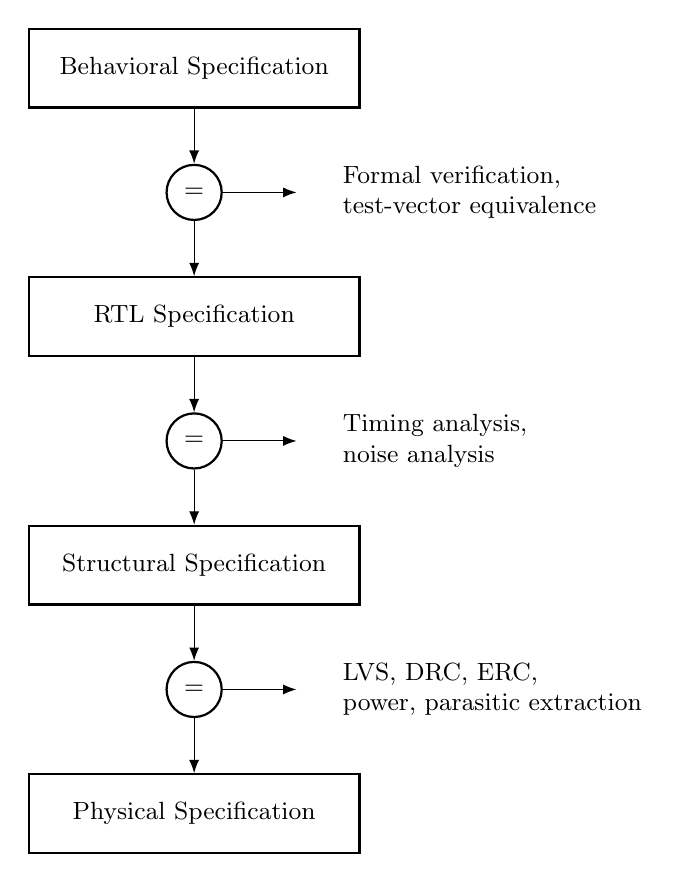
\begin{tikzpicture}[>=Latex, font=\small,
  lvl/.style={draw, thick, minimum width=4.2cm, minimum height=1cm, align=center},
  cmp/.style={draw, circle, thick, minimum size=0.7cm}]
\node[lvl] (b) {Behavioral Specification};
\node[cmp, below=0.7cm of b] (c1) {$=$};
\node[lvl, below=0.7cm of c1] (r) {RTL Specification};
\node[cmp, below=0.7cm of r] (c2) {$=$};
\node[lvl, below=0.7cm of c2] (s) {Structural Specification};
\node[cmp, below=0.7cm of s] (c3) {$=$};
\node[lvl, below=0.7cm of c3] (p) {Physical Specification};
\draw[->] (b) -- (c1); \draw[->] (c1) -- (r);
\draw[->] (r) -- (c2); \draw[->] (c2) -- (s);
\draw[->] (s) -- (c3); \draw[->] (c3) -- (p);
\node[right=1.4cm of c1, align=left] {Formal verification,\\ test-vector equivalence};
\node[right=1.4cm of c2, align=left] {Timing analysis,\\ noise analysis};
\node[right=1.4cm of c3, align=left] {LVS, DRC, ERC,\\ power, parasitic extraction};
\draw[->] (c1) -- ++(1.3,0); \draw[->] (c2) -- ++(1.3,0); \draw[->] (c3) -- ++(1.3,0);
\end{tikzpicture}
\end{document}
